\chapter{Kilika}

\begin{enumerate}
	\item \sd\ on exiting the boat, go up and left, \sd. \skippablefmv[2:00], (press Start immediately after skip) \sd
	\item Exit inn, go right to \wakka, \sd. Go left and up to Kilika Woods, \sd
\end{enumerate}
\begin{battle}{Lancet Tutorial}
	\begin{itemize}
		\item \sd
		      \kimahrif Lancet
		      \switch{\kimahri}{\yuna}
		      \yunaf Defend
		      \tidusf Attack
		      \luluf Fire
	\end{itemize}
\end{battle}
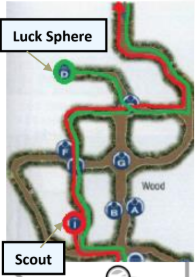
\includegraphics{graphics/kilikamap}
\begin{enumerate}[resume]
	\item Go left and up the hidden path, \pickup{Scout}
\end{enumerate}
\begin{spheregrid}
	\begin{itemize}
		\tidusf
		\begin{itemize}
			\item Move $\leftarrow\leftarrow$
			\item Flee, Agi+1
		\end{itemize}
	\end{itemize}
	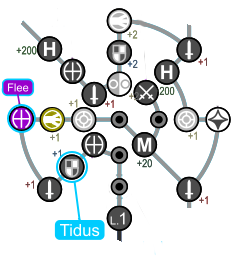
\includegraphics{graphics/Tidus_Kilika}
\end{spheregrid}
\begin{equip}
	\begin{itemize}
		\wakkaf Scout
		\item \textit{If you have them:}
		      \begin{itemize}
			      \wakkaf Ice Ball
			      \wakkaf Armguard
		      \end{itemize}
		\item \textit{If you got the Ice Brand:}
		      \begin{itemize}
			      \tidusf Ice Brand
		      \end{itemize}
	\end{itemize}
\end{equip}
\begin{enumerate}[resume]
	\item \formation{\tidus}{\yuna}{\wakka}
	\item Continue up the hidden path, following the map. Fill up \valefor\ \od\ with the first set, then do the rest of the encounters with the second set.
	\item Need 16 Speed Spheres from this point on. Need 45-55 AP on \tidus, which is about 5-7 kills.
\end{enumerate}
\bothvfill\winvfill\lossvfill
\begin{encounters}
	On Pre-Empts, Defend on Everyone.
	\begin{itemize}
		\item Killer Bee + Yellow Element:
		      \begin{itemize}
			      \tidusf Defend
			      \summon{\valefor}
			      \valeforf Boost
			      \valeforf Thunder Killer Bee
		            \valeforf Water Yellow Element
		      \end{itemize}
		\item Dinonix + Yellow Element
		      \begin{itemize}
			      \tidusf Attack Dinonix
			      \summon{\valefor}
			      \valeforf Boost x2
			      \valeforf Water Yellow Element
		      \end{itemize}
		\item Killer Bee + Dinonix + Yellow Element
		      \begin{itemize}
			      \tidusf Attack Dinonix
			      \summon{\valefor}
			      \valeforf Boost
			      \valeforf Thunder Killer Bee
			      \valeforf Water Yellow Element
		      \end{itemize}
		\item Killer Bee x2 + Ragora
			\begin{itemize}
				\tidusf Attack Ragora
				\summon{\valefor}
				\valeforf Thunder Killer Bee
				\valeforf Thunder Killer Bee
				\valeforf Fire x2 Ragora
			\end{itemize}
		\item Ragora (Bad Encounter)
		      \begin{itemize}
			      \tidusf Defend
			      \summon{\valefor}
			      \valeforf Boost
			      \valeforf Sonic Wings
			      \valeforf Fire x2
		      \end{itemize}
		\item 2x Ragora (Super Bad Encounter)
		      \begin{itemize}
			      \tidusf Defend
			      \summon{\valefor}
			      \valeforf Boost
			      \valeforf Dismiss
			      \wakkaf Defend
			      \item Flee
		      \end{itemize}
	\end{itemize}
\end{encounters}
\begin{encounters}
	\begin{itemize}
		\item Killer Bee: \wakka Attack
		\item Dinonix: \tidus\ Attack
		 \yunaf Defend
		\item Ragora: Flee
		\item Flee whatever is left.
	\end{itemize}
\end{encounters}
\begin{enumerate}[resume]
	\item \sd
	\item \formation{\tidus}{\yuna}{\wakka}
	\item \save
\end{enumerate}
\bothvfill\winvfill\lossvfill
\begin{battle}[3000]{Sinspawn Geneaux}
	\begin{itemize}
		\item \textit{If \tidus\ is going before \yuna:}
		      \begin{itemize}
			      \tidusf Attack Main Body
			      \summon{\valefor}
			      \valeforf Energy Blast \od
			      \valeforf Fire x4-5
		      \end{itemize}
		\item \textit{Else:}
		      \begin{itemize}
			      \switch{\yuna}{\kimahri}
			      \kimahrif Attack Main Body
			      \tidusf Defend
			      \switch{anyone}{\yuna}
			      \summon{\valefor}
			      \valeforf Energy Blast \od
			      \valeforf Fire x4
		      \end{itemize}
	\end{itemize}
Guaranteed 2 Power Spheres.
\end{battle}
\begin{enumerate}[resume]
	\item \sd\ on stone steps and temple. go into temple. Walk up to \wakka\ and Pray. \sd\ inside temple and go up steps. Wait for lift and \sd.
\end{enumerate}
\begin{trial}
	\begin{itemize}
		\item Take the sphere from the pedestal
		\item Place into the door, take it off of the door.
		\item Place sphere into the next door, take the sphere back.
		\item Place the sphere into the right holder
		\item Touch glpyh
		\item Take the sphere from the next room
		\item Place it into the left holder
		\item Take the glyph sphere from the pedestal
		\item Place it in the Fire Room
		\item Take the sphere that you put into the right holder
		\item Use it to open the door in the Fire Room
		\item Take the sphere off the door
		\item Enter the Fayth room
	\end{itemize}
\end{trial}
\begin{enumerate}[resume]
	\item In Fayth room, \sd, speak to \wakka\ first. Try to leave room, \sd, name \ifrit
	\item Hold down to exit temple, \cs[0:40], \sd
	\item Go south through Kilika Woods, take the left path and \pickup{Luck Sphere}, referencing map.
	\item Exit Kilika Woods same way that you entered, treating fights the same way as above.
	\item Go down and right to S.S. Winno. \sd
\end{enumerate}